\begin{frame}[t]
\frametitle{Balance del GNC}

\centering
{\small\color{blue!70!black}Fuente: MHCP y cálculos propios\par}
\vspace{0.2cm}
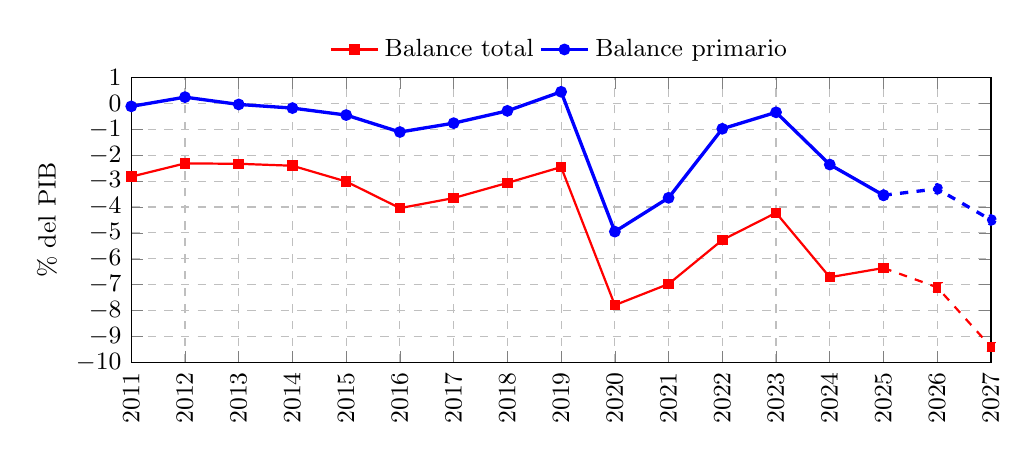
\begin{tikzpicture}
\begin{axis}[
    width=12.5cm, height=5.2cm,
    ylabel={\% del PIB},
    xmin=2011, xmax=2027,
    ymin=-10, ymax=1,
    xtick={2011,2012,...,2027},
    xticklabel style={rotate=90,anchor=east,/pgf/number format/.cd,1000 sep={},fixed,precision=0},
    scaled x ticks=false,
    scaled y ticks=false,
    ytick={-10,-9,...,1},
    tick label style={font=\small},
    ylabel style={font=\small},
    grid=major,
    grid style=dashed,
    legend style={at={(0.5,1.02)}, anchor=south, legend columns=2, font=\small, draw=none, fill=none},
    legend cell align=left
]

% Balance total, 2011--2025
\addplot[red, thick, mark=square*, mark size=1.5pt] coordinates {
    (2011,-2.828187579108)
    (2012,-2.316514744871)
    (2013,-2.331002797793)
    (2014,-2.406139599789)
    (2015,-3.015846864486)
    (2016,-4.04330349393)
    (2017,-3.654185677084)
    (2018,-3.069053994966)
    (2019,-2.457251637534)
    (2020,-7.788250635035)
    (2021,-6.971875007722)
    (2022,-5.273643973597)
    (2023,-4.223061232501)
    (2024,-6.710484245022)
    (2025,-6.354401832105)
};
\addlegendentry{Balance total}

% Balance primario, 2011--2025
\addplot[blue, very thick, mark=*, mark size=1.5pt] coordinates {
    (2011,-0.114508684913)
    (2012,0.241945750707)
    (2013,-0.039495846708)
    (2014,-0.180504894994)
    (2015,-0.450167769226)
    (2016,-1.104864015368)
    (2017,-0.76251975604)
    (2018,-0.287696033539)
    (2019,0.448259105264)
    (2020,-4.950256462957)
    (2021,-3.644991814951)
    (2022,-0.979875506563)
    (2023,-0.343875418705)
    (2024,-2.361646272935)
    (2025,-3.545012092036)
};
\addlegendentry{Balance primario}

% Proyecciones 2026--2027, conectadas con 2025
\addplot[red, thick, dashed, mark=square*, mark size=1.5pt, forget plot] coordinates {
    (2025,-6.354401832105)
    (2026,-7.1)
    (2027,-9.4)
};
\addplot[blue, very thick, dashed, mark=*, mark size=1.5pt, forget plot] coordinates {
    (2025,-3.545012092036)
    (2026,-3.3)
    (2027,-4.5)
};

\end{axis}
\end{tikzpicture}

\vspace{0.1cm}
{\scriptsize Líneas discontinuas: proyecciones para 2026 y 2027.\par}
\note{[Sources] Figuras.xlsx, hoja 1.4, B1:R3, versión del 17 de septiembre de 2026. Series: Balance\_Total y Balance\_Primario, 2011--2027, en porcentaje del PIB. Las líneas discontinuas corresponden a 2026 y 2027. La serie del balance primario coincide con Actualización y Consolidación de la hoja 4.2 hasta 2027.}
\end{frame}
